%Este trabalho está licenciado sob a Licença Atribuição-CompartilhaIgual 4.0 Internacional Creative Commons. Para visualizar uma cópia desta licença, visite http://creativecommons.org/licenses/by-sa/4.0/deed.pt_BR ou mande uma carta para Creative Commons, PO Box 1866, Mountain View, CA 94042, USA.

\chapter{Perceptron Multicamadas}\label{cap_mlp}
\thispagestyle{fancy}

\section{Modelo MLP}\label{cap_mlp_sec_modelo}

Uma Perceptron Multicamadas (MLP, do inglês, \textit{Multilayer Perceptron}) é um tipo de Rede Neural Artificial formada por composições de camadas de perceptrons. Consulte a Figura \ref{cap_mlp_sec_modelo}.

\begin{figure}[H]
  \centering
  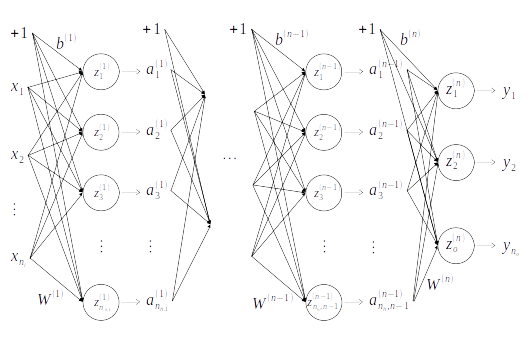
\includegraphics[width=\textwidth]{./cap_mlp/dados/fig_mlp/fig}
  \caption{Estrutura de uma rede do tipo Perceptron Multicamadas (MLP).}
  \label{fig:cap_mlp_sec_modelo:fig:mlp}
\end{figure}

Denotamos uma MLP de $n$ camadas por
\begin{align}
  \pmb{y} = \mathcal{N}\left(\pmb{x}; \left(W^{(l)}, \pmb{b}^{(l)}, f^{(l)}\right)_{l=1}^{n}\right),
\end{align}
onde $\left(W^{(l)}, \pmb{b}^{(l)}, f^{(l)}\right)$ é a tripa de pesos, bias e função de ativação da $l$-ésima camada da rede, $l=1, 2, \dotsc, n$.

A saída da rede é calculada por iteradas composições das camadas, i.e.
\begin{equation}
  \pmb{a}^{(l)} = f^{(l)}\underbrace{\left(W^{(l)}\pmb{a}^{(l-1)} + \pmb{b}^{(l-1)}\right)}_{\pmb{z}^{(l)}},
\end{equation}
para $l= 1, 2, \dotsc, n$, denotando $\pmb{a}^{(0)} := \pmb{x}$ e $\pmb{a}^{(n)} := \pmb{y}$.

\subsection{Treinamento}

Fornecido um conjunto de treinamento $\{\pmb{x}^{(s)}\}_{s=1}^{n_s}$, com $n_s$ amostras, o treinamento da rede consiste em resolver o problema de minimização
\begin{equation}
  \min_{(W,\pmb{b})}\varepsilon\left(\pmb{y}^{(s)}\right)
\end{equation}
onde $\varepsilon$ é uma dada função erro.

O problema de minimização pode ser resolvido por um \href{https://notaspedrok.com.br/notas/MatematicaNumericaAvancada/cap\_otimizacao_sec_minimi.html}{Método de Declive} e, de forma geral, consiste em:
\begin{enumerate}
\item $\pmb{w}, b$ aproximações iniciais.
\item Para $e\leftarrow 1, \dotsc, n_e$:
  \begin{enumerate}
  \item $\displaystyle (W, \pmb{b}) \leftarrow (W, \pmb{b}) - l_r\pmb{d}$
  \end{enumerate}
\end{enumerate}
onde, $n_e$ é o \emph{número de épocas}, $l_r$ é uma dada \emph{taxa de aprendizagem}\footnote{Em inglês, {\it learning rate}.} e o vetor direção $\pmb{d}$ depende dos gradientes
\begin{equation}
  \nabla_{W,\pmb{b}} \varepsilon := \left(\frac{\p\varepsilon}{\p W}, \frac{\p\varepsilon}{\p\pmb{b}}\right).
\end{equation}

O cálculo dos gradientes pode ser feito \emph{de trás para frente}, i.e. para os pesos da última camada, temos
\begin{align}
  \frac{\p\varepsilon}{\p W^{(n)}} &= \frac{\p\varepsilon}{\p\pmb{y}}\frac{\p\pmb{y}}{\p\pmb{z^{(n)}}}\frac{\p\pmb{z^{(n)}}}{\p W^{(n)}},\\
                             &= \frac{\p\varepsilon}{\p\pmb{y}}f'\left(W^{(n)}\pmb{a}^{(n-1)}+\pmb{b}^{(n)}\right)\pmb{a}^{(n-1)}.
\end{align}
Para os pesos da penúltima, temos
\begin{align}
  \frac{\p\varepsilon}{\p W^{(n-1)}} &= \frac{\p\varepsilon}{\p\pmb{y}}\frac{\p\pmb{y}}{\p\pmb{z^{(n)}}}\frac{\p\pmb{z^{(n)}}}{\p W^{(n-1)}},\\
                                     &= \frac{\p\varepsilon}{\p\pmb{y}}f'\left(\pmb{z}^{(n)}\right)\frac{\p\pmb{z}^{(n)}}{\p\pmb{a}^{(n-1)}}\frac{\p\pmb{a}^{(n-1)}}{\p\pmb{z}^{(n-1)}}\frac{\p\pmb{z}^{(n-1)}}{\p W^{(n-1)}}\\
                                     &= \frac{\p\varepsilon}{\p\pmb{y}}f'\left(\pmb{z}^{(n)}\right)W^{(n)}f'\left(\pmb{z}^{(n-1)}\right)\pmb{a}^{(n-2)}
\end{align}
e assim, sucessivamente para as demais camadas da rede. Os gradientes em relação aos \textit{biases} podem ser analogamente calculados.

\subsection{Aplicação: Problema de Classificação \texttt{XOR}}

Vamos desenvolver uma MLP que faça a operação $\texttt{xor}$ (ou exclusivo). I.e, receba como entrada dois valores lógicos $A_1$ e $A_2$ (V, verdadeiro ou F, falso) e forneça como saída o valor lógico $R = A_1 \texttt{xor} A_2$. Consultamos a seguinte tabela verdade:

\begin{center}
  \begin{tabular}{cc|c}
    $A_1$ & $A_2$ & $R$\\\hline
    V & V & F\\
    V & F & V\\
    F & V & V\\
    F & F & F\\\hline
  \end{tabular}
\end{center}

Assumindo $V = 1$ e $F = -1$, podemos modelar o problema tendo entradas $\pmb{x} = (x_1, x_2)$ e saída $y$ como na seguinte tabela:

\begin{center}
  \begin{tabular}{rr|r}
    $x_1$ & $x_2$ & $y$ \\\hline
    $1$ & $1$ & $-1$ \\
    $1$ & $-1$ & $1$ \\
    $-1$ & $1$ & $1$ \\
    $-1$ & $-1$ & $-1$ \\\hline
  \end{tabular}
\end{center}

\subsubsection{Modelo}

Vamos usar uma MLP de estrutura $2-2-1$ e com funções de ativação $f^{(1)}(\pmb{x}) = \tanh(\pmb{x})$ e $f^{(2)}(\pmb{x}) = id(\pmb{x})$. Ou seja, nossa rede tem duas entradas, uma camada escondida com 2 unidades (função de ativação tangente hiperbólica) e uma unidade de saída (função de ativação identidade).

\subsubsection{Treinamento}

Para o treinamento, vamos usar a função erro quadrático médio
\begin{equation}
  \varepsilon := \frac{1}{n_s}\sum_{s=1}^{n_s}\left|\tilde{y}^{(s)} - y^{(s)}\right|^2,
\end{equation}
onde os valores estimados $\tilde{y}^{(s)} = \mathcal{N}\left(\pmb{x}^{(s)}\right)$ e $\left\{\pmb{x}^{(s)}, y^{(s)}\right\}_{s=1}^{n_s}$, $n_s=4$, conforme na tabela acima.

\subsubsection{Implementação}

O seguinte código implementa a MLP e usa o Método do Gradiente Descendente (DG) no algoritmo de treinamento.

\lstinputlisting[caption=mlp\_xor.py, label=cap_mlp_sec_modelo:cod:mlp_xor]{./cap_mlp/dados/py_mlp_xor/main.py}

\subsection{Exercícios}

[[tag::construcao]]

\section{Aplicação: Aproximação de Funções}\label{cap_mlp_sec_apfun}

Redes Perceptron Multicamadas (MLP) são aproximadoras universais. Nesta seção, vamos aplicá-las na aproximação de funções uni- e bidimensionais.

\subsection{Função unidimensional}

Vamos criar uma MLP para aproximar a função gaussiana
\begin{equation}
  y = e^{-x^2},
\end{equation}
para $x\in [-1,1]$.

\lstinputlisting[caption=mlp\_gaussiana\_1d.py, label=cap_mlp_sec_modelo:cod:mlp_gaussiana_1d]{./cap_mlp/dados/py_mlp_gaussiana_1d/main.py}

\subsection{Função bidimensional}

Vamos criar uma MLP para aproximar a função gaussiana
\begin{equation}
  y = e^{-(x_1^2 + x_2^2)},
\end{equation}
para $\pmb{x} = (x_1, x_2)\in [-1,1]^2$.

\lstinputlisting[caption=mlp\_gaussiana\_2d.py, label=cap_mlp_sec_modelo:cod:mlp_gaussiana_2d]{./cap_mlp/dados/py_mlp_gaussiana_2d/main.py}

\subsection{Exercícios}

[[tag::construcao]]

\section{Aplicação: Equação de Laplace}\label{cap_mlp_sec_eqlaplace}

Vamos criar uma MLP para resolver
\begin{subequations}
  \begin{align}
    -\Delta u &= f,\quad \pmb{x}\in D = (-1, 1)^2,\\
    u &= 0,\quad \pmb{x}\in\p D.
  \end{align}
\end{subequations}

Para validação, vamos considerar um problema com solução manufaturada
\begin{equation}
  u(\pmb{x}) = \sen(\pi x_1)\sen(\pi x_2)
\end{equation}
o que nos fornece
\begin{equation}
  f = \pi^2\sen(\pi x_1)\sen(\pi x_2).
\end{equation}

[[tag::construcao]]

\subsection{Exercícios}

[[tag::construcao]]
